 \let\negmedspace\undefined
\let\negthickspace\undefined
\documentclass[journal]{IEEEtran}
\usepackage[a5paper, margin=10mm, onecolumn]{geometry}
\usepackage{lmodern} % Ensure lmodern is loaded for pdflatex
\usepackage{tfrupee} % Include tfrupee package

\setlength{\headheight}{1cm} % Set the height of the header box
\setlength{\headsep}{0mm}     % Set the distance between the header box and the top of the text

\usepackage{gvv-book}
\usepackage{gvv}
\usepackage{cite}
\usepackage{amsmath,amssymb,amsfonts,amsthm}
\usepackage{algorithmic}
\usepackage{graphicx}
\usepackage{textcomp}
\usepackage{xcolor}
\usepackage{txfonts}
\usepackage{listings}
\usepackage{enumitem}
\usepackage{mathtools}
\usepackage{gensymb}
\usepackage{comment}
\usepackage[breaklinks=true]{hyperref}
\usepackage{tkz-euclide} 
\usepackage{listings}
\usepackage{gvv}                                        
\def\inputGnumericTable{}                       
\usepackage[latin1]{inputenc}                                
\usepackage{color}                                            
\usepackage{array}                                            
\usepackage{longtable}                                       
\usepackage{calc}                                             
\usepackage{multirow}                                         
\usepackage{hhline}                                           
\usepackage{ifthen}                                           
\usepackage{lscape}  
\usetikzlibrary{patterns}
\begin{document}
\bibliographystyle{IEEEtran}


\textbf{Question 4.8.22:} \\
The distance of the line 
\begin{align}
\vec{r} = (\hat{i} - \hat{j}) + \lambda(\hat{i} + 5\hat{j} + \hat{k})
\end{align}
from the plane 
\begin{align}
\vec{r} \cdot (\hat{i} - \hat{j} + 4\hat{k}) = 5
\end{align}
is \, ?

\textbf{Solution:}

Let the line be given as:
\begin{align}
\vec{r} = \myvec{1 \\ -1 \\ 0} + \lambda \myvec{1 \\ 5 \\ 1} \label{1}
\end{align}

Let the plane be:
\begin{align}
\vec{r}^\top \myvec{1 \\ -1 \\ 4} = 5 \label{2}
\end{align}

Let:
\begin{align}
\vec{a} = \myvec{1 \\ -1 \\ 0}, \quad \vec{m} = \myvec{1 \\ 5 \\ 1}, \quad \vec{n} = \myvec{1 \\ -1 \\ 4} \label{3}
\end{align}

The direction vector \( \vec{m} \) is along the line.  
The normal vector \( \vec{n} \) is normal to the plane.

\textbf{Step 2: Compute \( \vec{m}^\top \vec{n} \)}

\begin{align}
\vec{m}^\top \vec{n} = \myvec{1 & 5 & 1} \myvec{1 \\ -1 \\ 4} = 1 - 5 + 4 = 0 \label{7}
\end{align}


So, the line is **parallel to the plane** and does **not intersect**.

---

Now, we use **distance from point to plane** formula geometrically.

Since line is parallel to the plane, the perpendicular distance from **any point** on the line to the plane is the required distance.

Let us choose \( \vec{a} = \myvec{1 \\ -1 \\ 0} \)

Let \( d \) be the distance from point \( \vec{a} \) to the plane.

Let the distance be:
\begin{align}
d = \frac{| \vec{a}^\top \vec{n} - 5 |}{\sqrt{ \vec{n}^\top \vec{n} }} \label{9}
\end{align}



Compute \( \vec{n}^\top \vec{n} \):
\begin{align}
\vec{n}^\top \vec{n} = \myvec{1 & -1 & 4} \myvec{1 \\ -1 \\ 4} = 1 + 1 + 16 = 18 \label{10}
\end{align}

Therefore:
\begin{align}
d = \frac{|2 - 5|}{\sqrt{18}} = \frac{3}{\sqrt{18}} = \frac{3}{3\sqrt{2}} = \frac{1}{\sqrt{2}} \label{11}
\end{align}

\[
\boxed{d = \frac{1}{\sqrt{2}}}
\]
\newpage
\begin{figure}[h!]
    \centering
    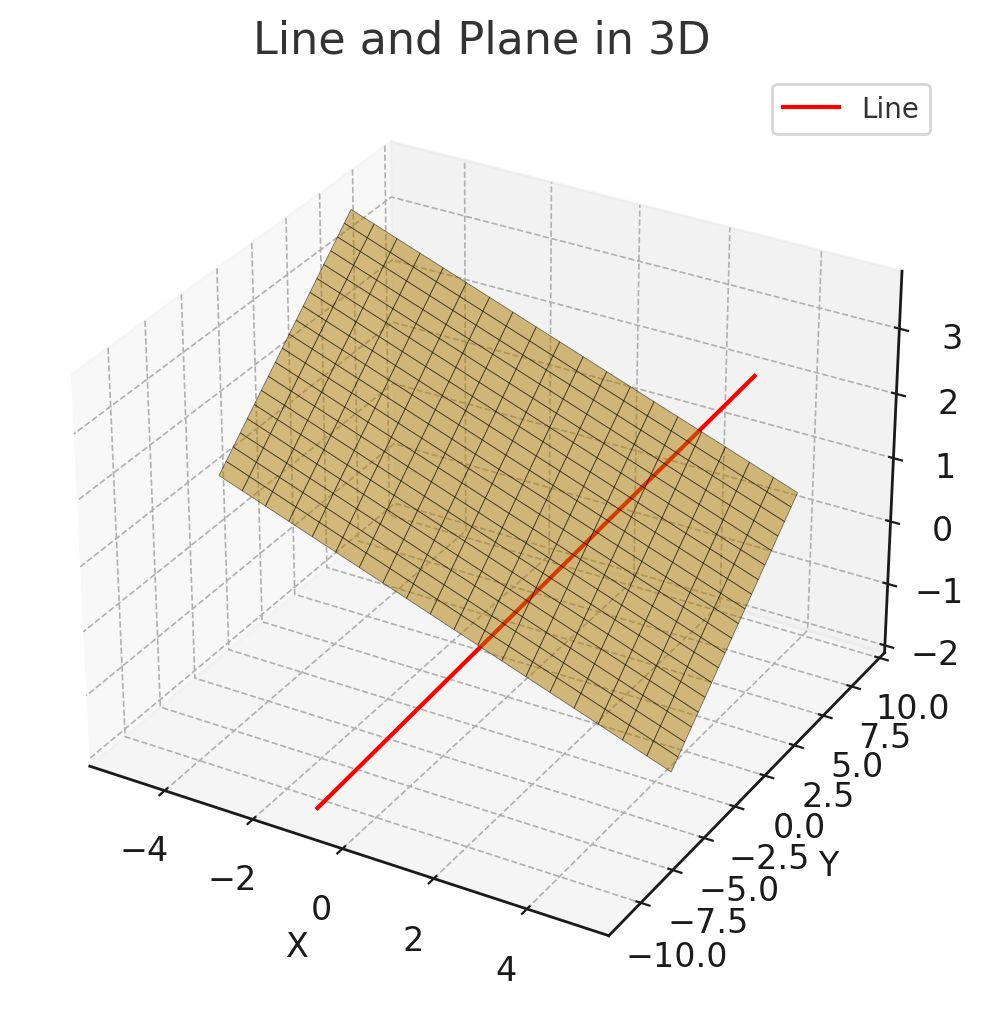
\includegraphics[width=0.5\linewidth]{figs/mat8.jpeg}
    \caption{Caption}
    \label{fig:placeholder}
\end{figure}
\end{document}

